\documentclass[10pt,twocolumn,letterpaper]{article}

\usepackage{cvpr}
\usepackage{times}
\usepackage{epsfig}
\usepackage{graphicx}
\usepackage{amsmath}
\usepackage{amssymb}




% Include other packages here, before hyperref.

% If you comment hyperref and then uncomment it, you should delete
% egpaper.aux before re-running latex.  (Or just hit 'q' on the first latex
% run, let it finish, and you should be clear).
\usepackage[breaklinks=true,bookmarks=false]{hyperref}

\cvprfinalcopy % *** Uncomment this line for the final submission

\def\cvprPaperID{****} % *** Enter the CVPR Paper ID here
\def\httilde{\mbox{\tt\raisebox{-.5ex}{\symbol{126}}}}

% Pages are numbered in submission mode, and unnumbered in camera-ready
%\ifcvprfinal\pagestyle{empty}\fi
\setcounter{page}{4321}
\begin{document}

%%%%%%%%% TITLE
\title{Personalized Smart Display }

\author{Eddie Dounn\\
Intro ML\\
CS4347\\
{\tt\small eid1@txstate.edu}
% For a paper whose authors are all at the same institution,
% omit the following lines up until the closing ``}''.
% Additional authors and addresses can be added with ``\and'',
% just like the second author.
% To save space, use either the email address or home page, not both

}

\maketitle
%\thispagestyle{empty}

%%%%%%%%% ABSTRACT
\begin{abstract}
   To expand on the traditional Smart Display/Smart Mirror systems to not only provide common areas quick information but also for individual users.  This system would use facial detection methods to recognize users to provide personalized information.  When no users are detected the traditional system would provide generic information.  This provides a level of personalizing for multiple people in a common household or work area as well as can be expanded on for other needs such as security. 
\end{abstract}

%%%%%%%%% BODY TEXT
\section{Introduction}

Expanding on the traditional Smart Display/Smart Mirror systems designed for homes and small offices.  These systems usually provide generic information such as the time, the weather, calendar, and upcoming events.  The scope of my project is to provide a system to allow for penalization of these systems.  The use of facial detection methods provides a way for the display to know which user it should be display information for.  On this project I'm expanding on this smart display idea and implementing it with web technologies (javascript) for a more customized implementation.  This also allows it to be implemented in such open source smart display frameworks such as Magic Mirror.  I have chosen to use Face-api.js for the face detection implementation as it uses multiple face detection models though tensorflow.js core API.  It is also developed in javascript which makes it easy to implement into a custom made smart display or into open source projects such as the web centered Magic Mirror. 

%-------------------------------------------------------------------------
\subsection{Problem}

I wanted to expand on the traditional smart displays as the implementation of those systems are designed for a general use case with each person looking at the same information.  This project still allows for general information to be shown in a traditional manner as well as personalized information for users in the system.

\subsection{Code Language}

Many open source smart display projects are using node.js for their smart display framework.  Thus, I chose to use javascript and nodejs to implement Face.api.  This makes it easier to implement this into the existing traditional smart display frameworks.\cite{Stephen}

\subsection{Further Expansion}
My expansion on the traditional smart display requires a camera for face detection. The addition of this hard ware leads to many other additions.  Face-api.js detects emotions via face detection, opening up further possibilities to expand on.  The addition to a camera to the hardware opens up other possibilities such as object detection, monitoring for pets, and face detection for security.


%-------------------------------------------------------------------------
\subsection{Project Code}

Code for this entire project can be found at \url{https://github.com/edounn/cs4347}

\section{Face Detection}

Using TensorFlow and Face-api.js one has access to a few different face detection models.  The one chosen for this project was Single Shot Multibox Detector or SSD.  This is a neural net that computes the locations of each face in an image.  This provides us with the ability to detect one or more face.  This could allow a user to setup a more secure smart display, showing private information only if no other face is detected. 

%-------------------------------------------------------------------------
\subsection{Model selection}

For face detection, this project implements a SSD (Single Shot Multibox Detector) based on MobileNetV1. The neural net will compute the locations of each face in an image and will return the bounding boxes together with it's probability for each face. Once the face has been detected it can pass the name to a database and pull the settings for this user to know what information to display.   This face detector is aiming towards obtaining high accuracy in detecting face bounding boxes instead of low inference time. \cite{face-api}


%-------------------------------------------------------------------------
\subsection{SSD Mobilenet}

This project uses the Single Shot Multibox Detector or SSD mobilenet model. Some information about the architecture: \cite{Muhler}

Single shot:  means that the task of object localization and classification are done in a single forward pass of the network.

MultiBox:  A name of a bounding box regression technique.

Detector:  The network is an object detection that also classifies those detected objects.

Confidence Loss: this measures how confident the network is of the objects of the computed bounding box. Categorical cross-entropy is used to compute this loss.

Location Loss: this measures how far away the network’s predicted bounding boxes are from the training set.

\begin{center} multibox loss = confidence loss + alpha * location loss \end{center}


The alpha term helps in balancing the contribution of the location loss.  The goal in this would be to find the parameter values that most reduce the loss function.

For this project the SSD mobilenet model is handled by Tensorflow.
\begin{figure}
\begin{center}
\fbox{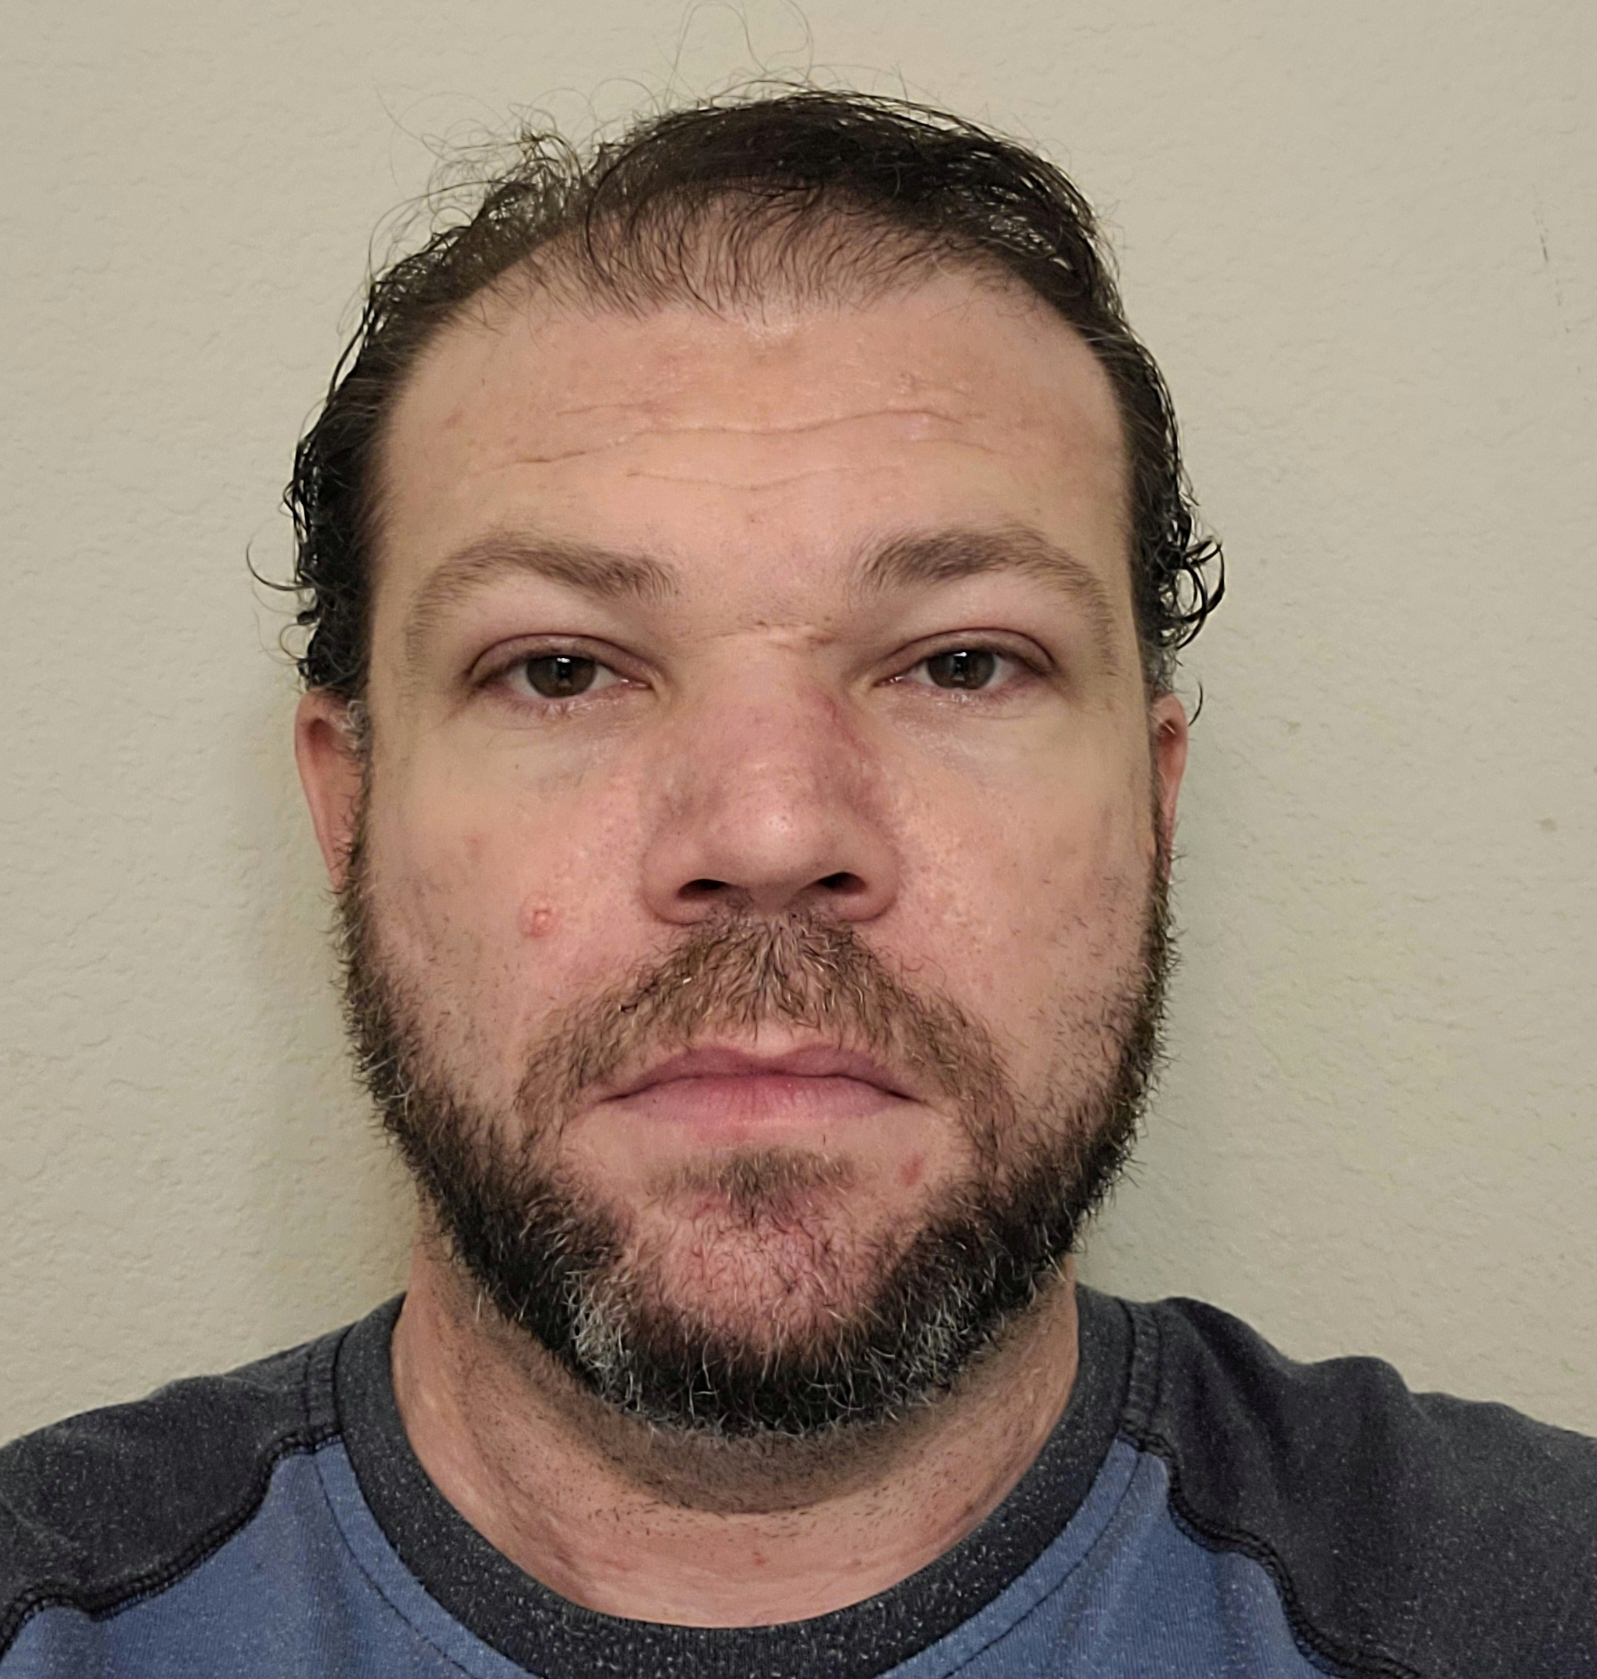
\includegraphics[width=0.8\linewidth]{eddie.jpeg}   }
\end{center}
   \caption{My personal user picture passed to the model.}
\label{fig:long}
\label{fig:onecol}
\end{figure}

%------------------------------------------------------------------------

\subsection{System users}

Each user for this system would need an identifying picture. Such as my example \ref{fig:onecol}.  Once the confidence number is high enough the system reads the name of the file and renders a box with the picture text over the image, as done in our example.  However, for the smart display module I instead opted out of displaying the image and used the descriptor name as key to that users settings.  Providing a way to display everything for that user.

For this project each user has a folder where their picture is placed.  From here the picture processed with Tensorflow's models.  Other models can also use the same folder format.
\begin{figure}
\begin{center}
\fbox{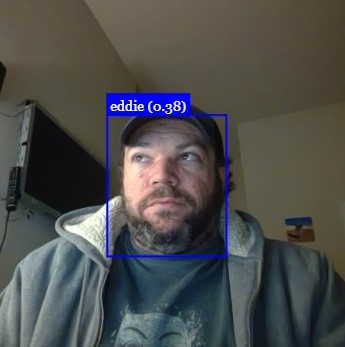
\includegraphics[width=0.8\linewidth]{screenshot.jpg}   }
\end{center}
   \caption{Example of detection accuracy and name overlaid on webcam output.}
\label{fig:long}
\label{fig:onecol}
\end{figure}

%------------------------------------------------------------------------
\section{Results}

During this project it started to become apparent that the Raspberry Pi was struggling to process the webcam video while managing the face-api processes.  Raising the amount of time for each frame did help.  The initial loading time for for the model is slow but after loaded it can detect faces at a decent speed.  Moving to the other models did work, but did not produce the results I wanted.  Some models detected only points on a face.  The other face recognition models could only locate one face at a time and had a lower accuracy.




%------------------------------------------------------------------------
\section{Final Ideas}

I'm excited to continue working on this project.  I intend to create a back-end system that allows someone to add and remove users and also allow users to modify what they'd shown when the display detects them. 




{\small
\bibliographystyle{ieee}
\bibliography{resources}
}


\end{document}
